\section{Deduplication Analysis}
\label{sec:dedup}

\subsection{File level deduplication ratio}

\subsubsection{Redundant file overhead in terms of file repeat count and redundant storage overhead}


\begin{figure}
	\centering
	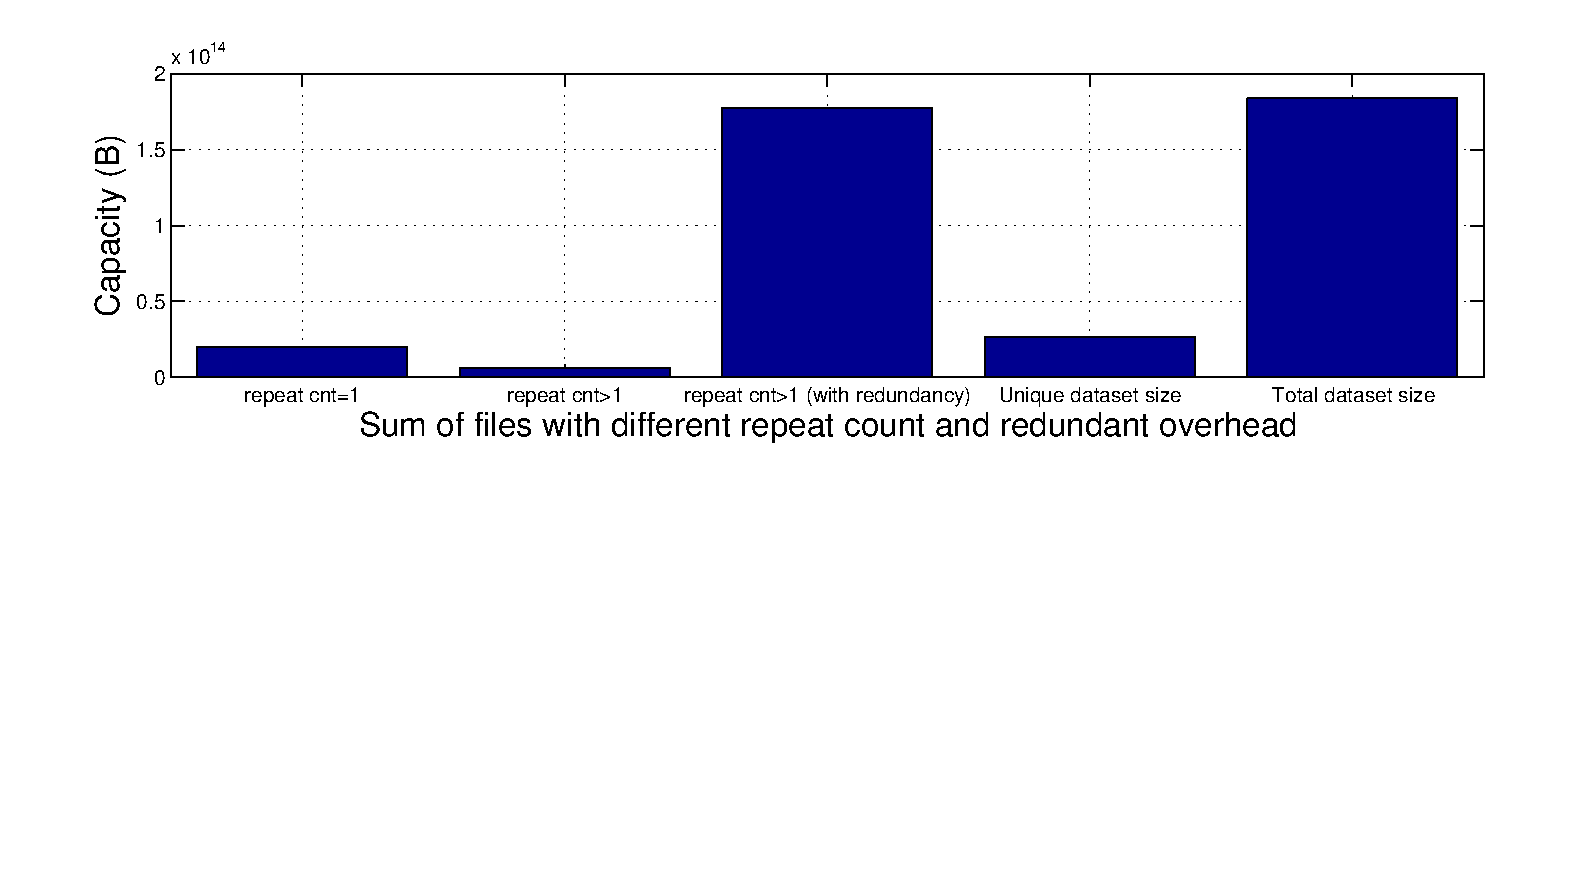
\includegraphics[width=0.5\textwidth]{graphs/capacity_data_ratio.eps}
	\caption{Redundant storage overhead.
	}
	\label{fig_redundant_overhead}
\end{figure}

\begin{table} 
	\centering 
	\scriptsize  
	%\begin{minipage}{.5\linewidth}
	\caption{Redundant ratio in terms of file count and capacity} \label{tbl:schemes} 
	\begin{tabular}{|l|l|l|}%p{0.14\textwidth} 
		\hline 
		% after \\: \hline or \cline{col1-col2} \cline{col3-col4} ... 
		% after \\: \hline or \cline{col1-col2} \cline{col3-col4} ... 
		       & File count & Capacity \\
		\hline
		Repeat cnt = 1 & 0.58\% & 10.87\%\\
		\hline
		Repeat cnt $>$ 1 after dedup & 2.59\% & 3.44\%\\
		\hline
		Repeat cnt $>$ 1 before dedup  & 99.42\%  & 89.13\%\\
		\hline
		Unique dataset & 3.17\% (167,251,437)  &  14.31\% (23.92 TB) \\
		\hline 
		Total dataset & 5,278,465,130 & 167.20 TB \\
		\hline 	
		%\hline 
	\end{tabular} 
\end{table} 

\paragraph{File repeat count distribution.}

Almost 90\% of files have equal or less than 10 redundant copies. Most files have small repeat count.

\begin{figure}
	\centering
	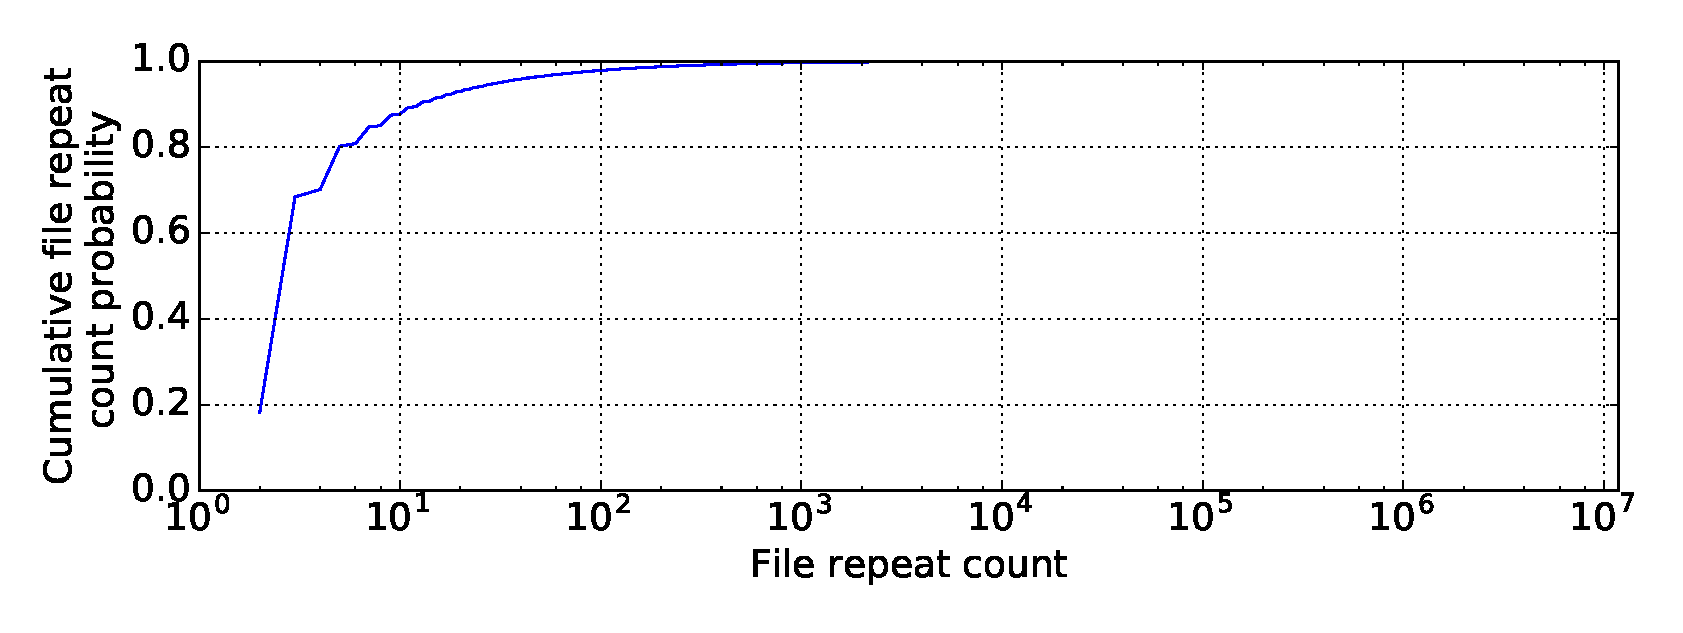
\includegraphics[width=0.5\textwidth]{graphs/File_repeat_count.eps}
	\caption{CDF of file repeat count.
	}
	\label{fig_file_repeat_count}
\end{figure}

\paragraph{Unique file size distribution.}

91\% files'sizes are equal or less than 100KB. Most files are smaller files.

\begin{figure}
	\centering
	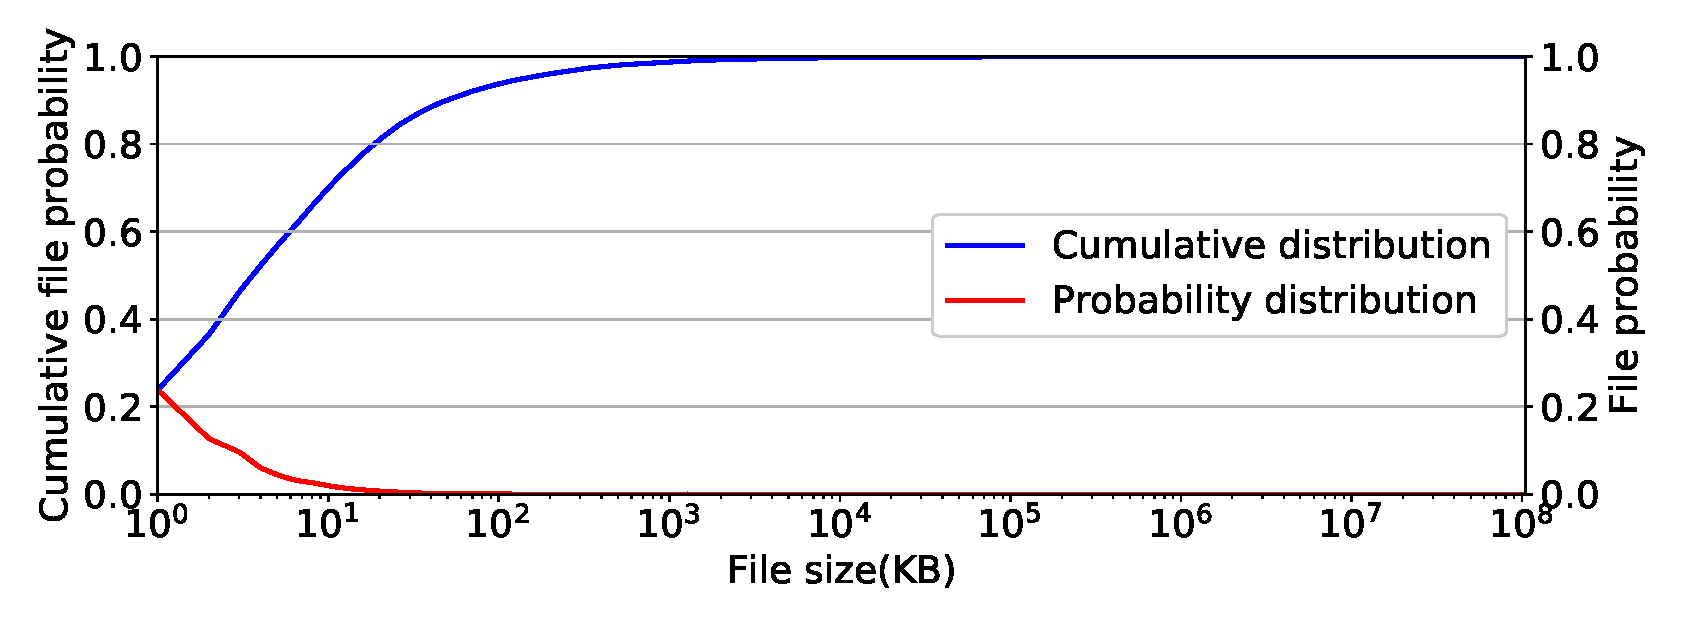
\includegraphics[width=0.5\textwidth]{graphs/File_size-KB.eps}
	\caption{CDF of unique file size (KB).
	}
	\label{fig_file_size}
\end{figure}

\paragraph{Redundant file storage overhead.}

Total size of redundant files with same content(TRS)

97\% of the TRSs are equal or less than 100MB.

\begin{figure}
	\centering
	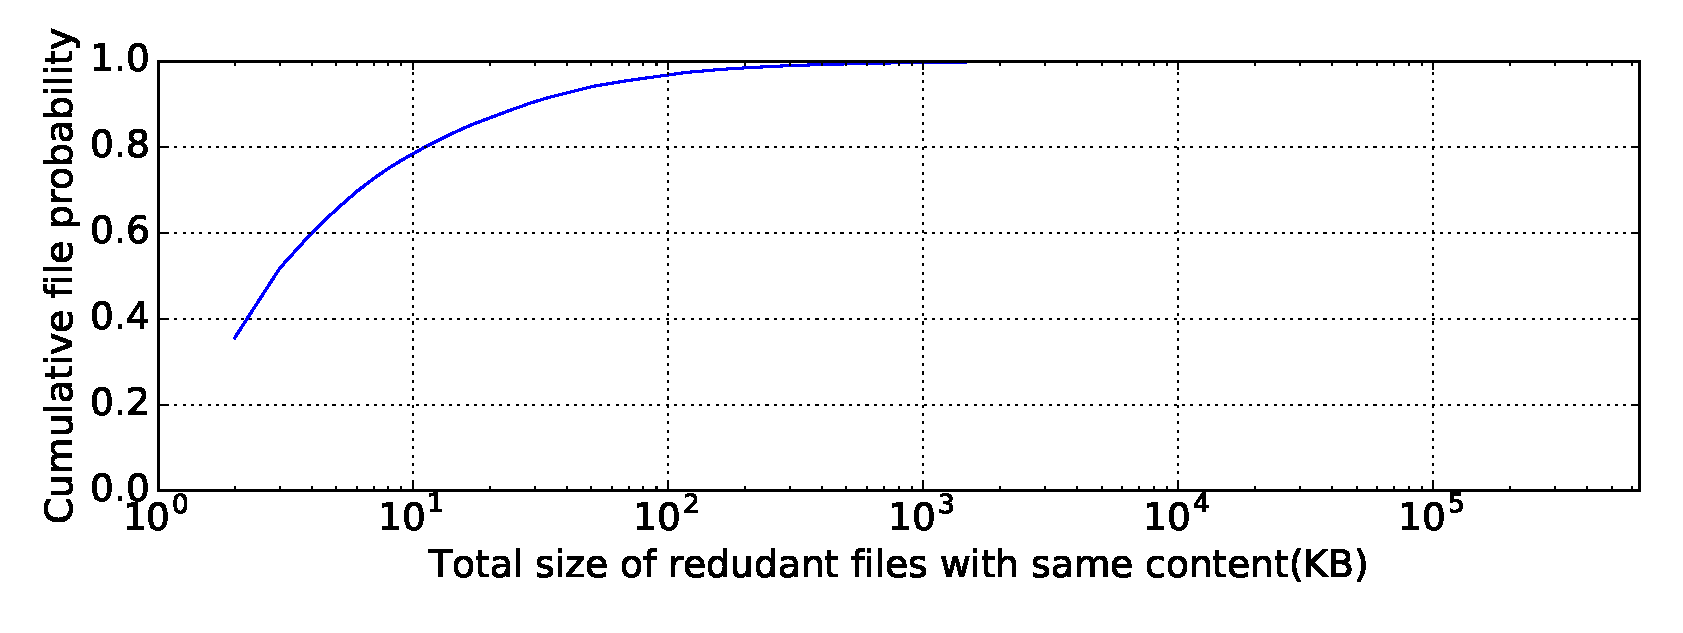
\includegraphics[width=0.5\textwidth]{graphs/Total_size_of_redudant_files_with_same_content-KB.eps}
	\caption{CDF of total file size with same file content (MB).
	}
	\label{fig_total_redundant_same_digest}
\end{figure}

\paragraph{Average file size by repeat count.}

There is no relation between file repeat count and average file size.

\begin{figure}
	\centering
	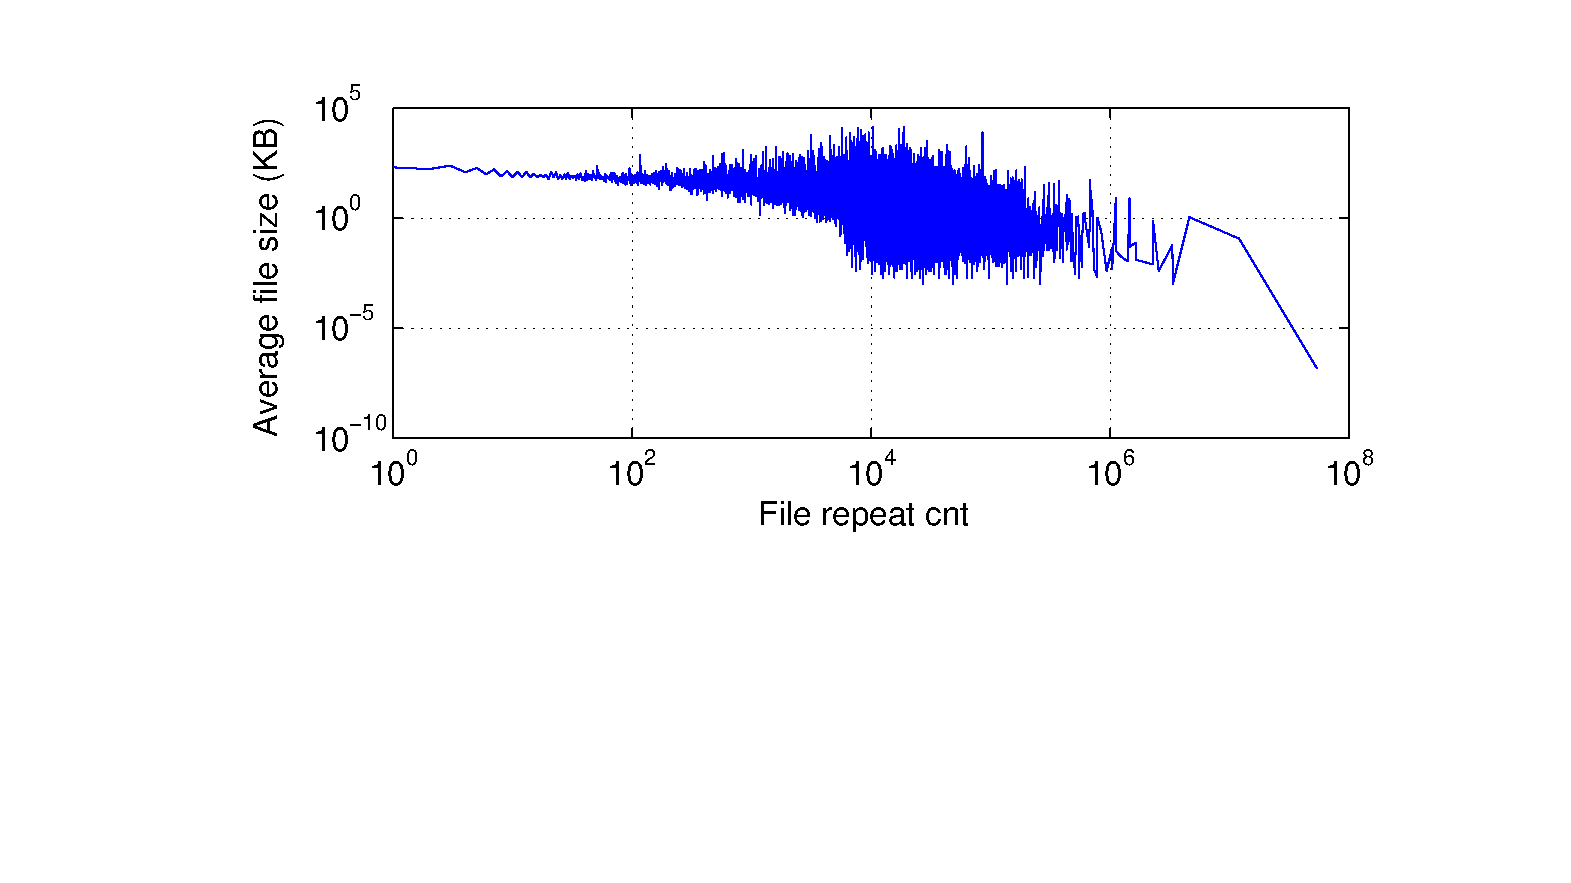
\includegraphics[width=0.5\textwidth]{graphs/avg_size_by_cnt.eps}
	\caption{Average file size with same repeat count.
	}
	\label{fig_avg_size_by_cnt}
\end{figure}

\paragraph{Total file size by repeat count.}

However, with the increase of file repeat count, the sum of file size with same repeat count becomes smaller.

\begin{figure}
	\centering
	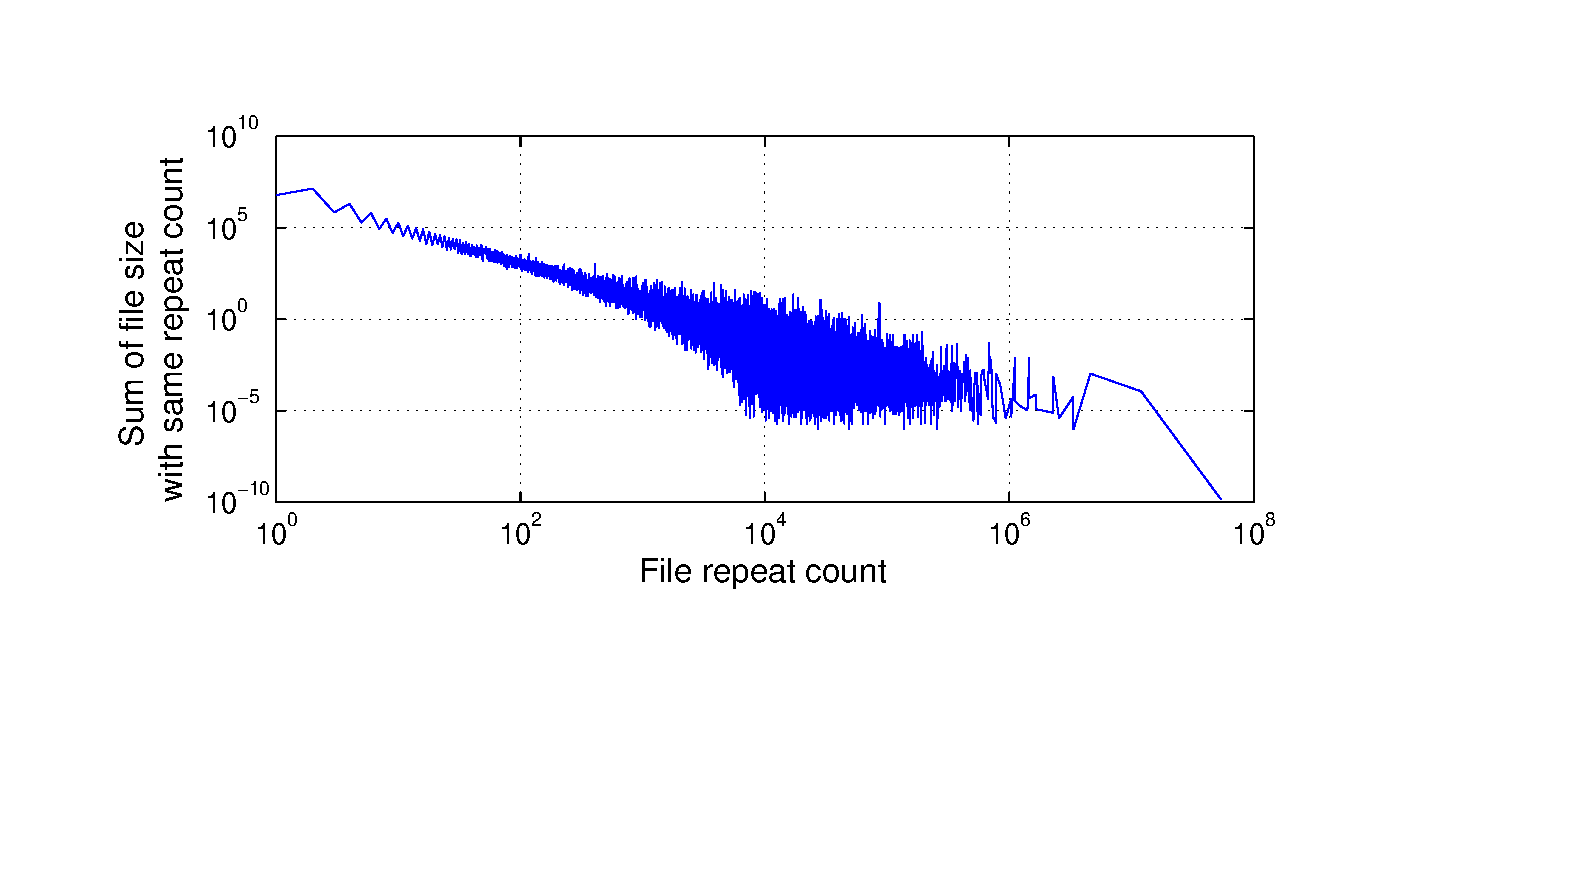
\includegraphics[width=0.5\textwidth]{graphs/sum_size_by_cnt.eps}
	\caption{Sum of file size with same repeat count.
	}
	\label{fig_sum_by_cnt}
\end{figure}

\subsubsection{What are the redundant files?}


\paragraph{File type distribution.}


\paragraph{File functionality distribution.}


\paragraph{File age distribution.}


\subsection{Suggest 1: File-Level Content Addressable Storage Model}


\subsection{Redundant files in layers}


\subsubsection{Redundant storage overhead for individual layers}


\subsubsection{Redundant storage overhead across layers}


\subsubsection{Why do layers have so many redundant files?}


\subsection{Redundant files in images}

%\subsubsection{Redundant file characterization}

\subsection{Chunking Deduplication}

\subsubsection{Chunking Deduplication ratio}
